\textbf{Electroweak Unification}

\todo[inline]{understand the different polarization things for W}

\begin{center}
    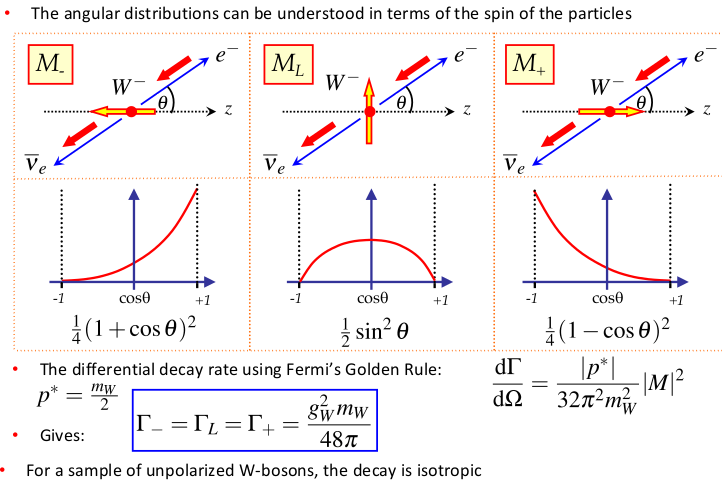
\includegraphics[width=\linewidth]{images/w_decays.png}

    $\Gamma(W^- \to e^- \bar{\nu}_e) = \frac{g_W^2 m_W}{48\pi}$

    (multipliers below are relative to this)

    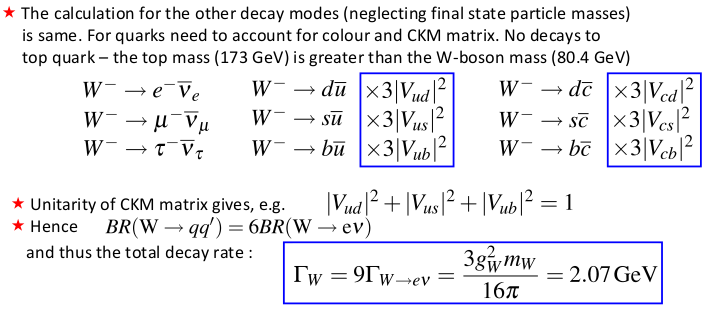
\includegraphics[width=\linewidth]{images/w_quark_decays.png}
\end{center}
Local gauge transformation of QED: SU(2) trans. $\phi' = \phi e^{i\vec{\alpha}(x) \cdot \frac{\vec{\sigma}}{2}}$

Generators: Pauli matrices, $\alpha_i(x)$ = local phases, give 3 gauge bosons, $W_1^\mu, W_2^\mu, W_3^\mu$.

$W^\pm = \frac{1}{\sqrt{2}} \left(W^1 \mp W^2\right)$

\begin{center}
    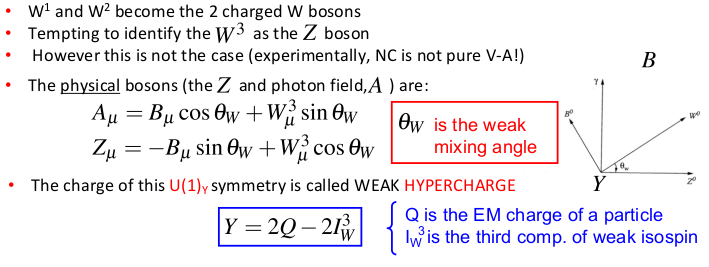
\includegraphics[width=\linewidth]{images/ew_unification.png}
\end{center}

Overall EW Unification Idea:

$U(1)_{EM} \implies$ QED

$SU(2)_{L} \implies W_1, W_2 = W^\pm, W_3$

$SU(3)_{col} \implies$ QCD

If you introduce $U(1)_Y \implies B_\mu$ you can unify EM \& weak.

Once $\theta_W$ is known, properties of Z are determined.

Experimentally, roughly, $\sin^2(\theta_W) = 0.23$

Z couples to left- and right-handed chiral states but not equally.

$I_W$ = weak isospin, neutrinos have $1/2$ leptons have $-1/2$

\begin{center}
    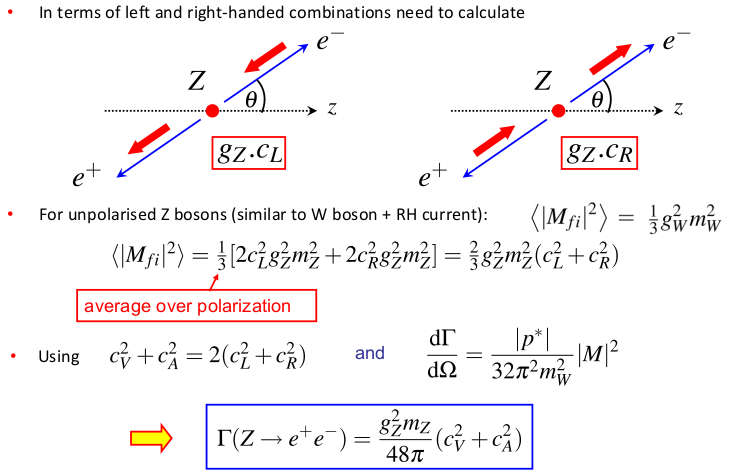
\includegraphics[width=\linewidth]{images/z_decays.png}
    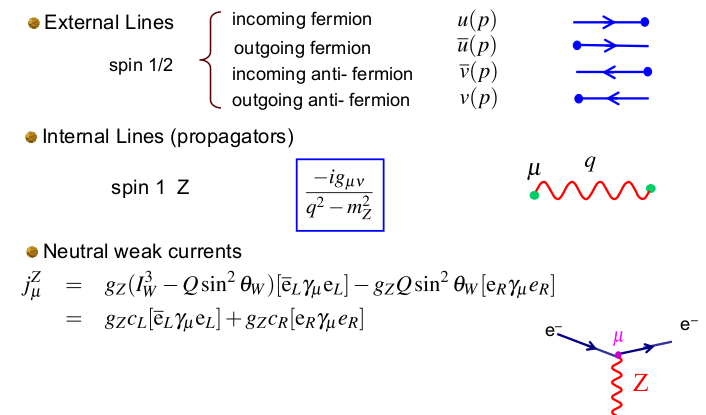
\includegraphics[width=\linewidth]{images/neutral_current_feynrules.png}
    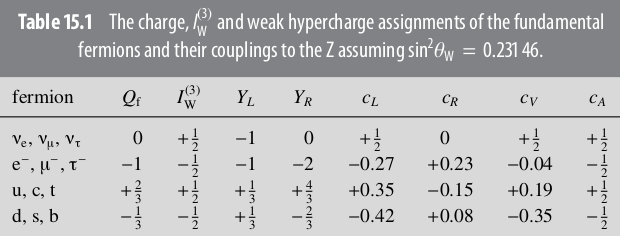
\includegraphics[width=\linewidth]{images/z_coupling_params.png}
\end{center}
